\documentclass[conference]{IEEEtran}
%\usepackage{cite}
\usepackage[pdftex]{graphicx}
%\graphicspath{{images/}}
\DeclareGraphicsExtensions{.pdf}
\usepackage{array}
\usepackage{url}
\usepackage{amsmath}

% correct bad hyphenation here
%\hyphenation{}

\begin{document}
\title{Drinking from the Firehose: Engineering vs.Theory in Wireless
  Power Management}

\author{\IEEEauthorblockN{Nicholas Farnan and James Larkby-Lahet}
\IEEEauthorblockA{Department of Computer Science, University of Pittsburgh\\ Pittsburgh, PA 15260 -- USA \\ Email: \{nlf4,jamesll\}@cs.pitt.edu}}
\maketitle

\section{Introduction}

Frequently, when we think of networks in the abstract, we imagine two
symmetric channels between nodes.  However engineering realities often
lead us to the design of asymmetric communication pathways, common
examples include DSL and cable broadband which can provide download
speeds in excess of 16 times the maximum upload speed.

In wireless networks we can also encounter asymmetric channels,
sometimes due to heterogeneity of hardware or environment (for
example, in the face of interference wifi devices can reduce their
transmission rate).

We decided to examine a somewhat different problem.  We were curious
whether we could reduce the transmission speeds of wireless,
battery-powered nodes and then use the high-bandwidth downlink from
a line-powered base station in some manner to reduce the number of
bits that must be uploaded across the slow link.

In the next section we discuss an instructive toy problem environment
which motivated our research in this area.  In section 3 we discuss
our implementation of an asymmetric communication protocol.  In
section 4 we present results and discuss why we were unable to
achieve positive results with this approach.

\section{Background}

First we examine a relaxation of the wireless communication
environment we wish to improve.  Instead, imagine a 2 node serial
network, with a single serial communication channel from each node to
its partner.  One of these channels, which we will dub the downlink,
runs at a rate significantly faster than the other.  For concreteness
let us say the downlink is capable of 16 bits per second and the
uplink is limited to 1 bit per second.

In this setting, we can think about what could be transmitted by the
downlink in order to reduce the number of bits sent via the uplink.
One option would be to transmit guesses along the downlink (from the
`server') as to what the uplink using `client' wishes to transmit.
When the client receives a guess that matches its data, it can respond
with a single bit acknowledgment, provided the server can calculate
backward from receipt to determine which guess is indicated by the ACK.

\section{Related Work}
This section has been omitted as it is covered in the other paper.

\section{Implementation}
We attempted to take the guess and ACK protocol, which we refer to as
`The Firehose', and apply it to packetized communication.  Since
packets may contain much more than the 3 to 8-bit guess sizes we
intended to use, and since the IP overhead is at least 20 bytes, we
needed to transmit a number of guesses in the same packet and
acknowledge more than a single group at a time.

We refer to the set of groups actively undergoing discovery via the
firehose protocol as the `frame'.  The server always transmits a
full frame's worth of data, and while the client attempts to send as
few bits in acknowledgment (or none at all if the guesses are all
wrong) as possible.  However, since the ACK is a bitmap with 1's
indicating correct guesses, we frequently end up sending 0's, implicit
NACKs, which greatly increases our client transmission overhead, as we
will see.

When guesses are acknowledged, the server replaces the range of bits
in the Frame reserved for the ACKed guess with a guess for a new range
of bits in the file.  The next guess packet issued by the server
includes a sequence number that the client uses to coordinate updates
to its Frame in sync with the server.

After an initial implementation to demonstrate that this scheme could
actually be used to transfer information, we moved on to trying to
reduce the number of bytes transmitted and received by the client, in
order to reduce the energy usage of our scheme.

\subsection{Guess Models}
Our initial attempt to reduce the number of bits transceived by the
client was to modify how guesses are issued.  Initially we had been
using a deterministic model which always guessed 0 through N in order.
We decided that adaptive guess models, attempting to capture patterns
in the workload, might be able to reduce our power consumption in two
ways.  The first batch of savings comes from that fact that if correct
guesses are issued earlier, fewer incorrect guesses must be issued and
therefore fewer bits are received by the client.  The second batch of
savings comes from the fact that if fewer incorrect guesses are
received, there is less opportunity for the client to be forced to
transmit NACK placeholders, and therefore fewer bits will be sent.

We implemented 8 guess models.  For zero information models,
Deterministic was joined by Random, which selected a random guess
ordering for each new group of bits added to the Frame.  We also
implemented a Most Frequently Used and Most Recently Used model, since
MFU is essentially the ordering used by optimal entropy encoders, we
expected it to perform well, but we thought that recency might allow
us to take advantage of spatial locality within the file.

Using the same intuitions we also implemented Least Frequently and
Least Recently NACKed experts, attempting to turn the undesired NACK
bits we were receiving anyhow into useful information.  We also
implemented Most Frequently ACK/NACKed, which used the ratio of ACKs
to NACKs as its `goodness' metric.

For our final Guess Model we implemented a Weighted Majority machine
learning algorithm, with our other models serving as experts.  The
idea here is that the learning algorithm may be able to switch models
in response to the `workload' and also that several of our poorer quality
experts might still have proven valuable when choices than many of
them agreed on could be chosen without having to act on the less
sensible `loner' suggestions of the model.


\subsection{ACK Encodings}

We also attempted to change representations of our ACKs via several
schemes.  The first choice considered was whether to send an ACK or
NACK, that is, whether to treat ones or zeros as data.  We then
attempted to trim the 'non-data' from either the back or front of the
packet, in whichever manner provided greater savings.  We then
compared the trimmed ACK and NACK representations to Index and
run-length encoded versions of themselves.  The former being an array
of the indexes of the data bits in the ACK or NACK, counting from the
non-trimmed side of the bitmap, and the later being a list of $(index,
length)$ pairs encoding the index of all data bits preceded by a
non-data bit, and the number of consecutive data bits following. 

\section{Results}

\begin{figure}[!t]
\centering
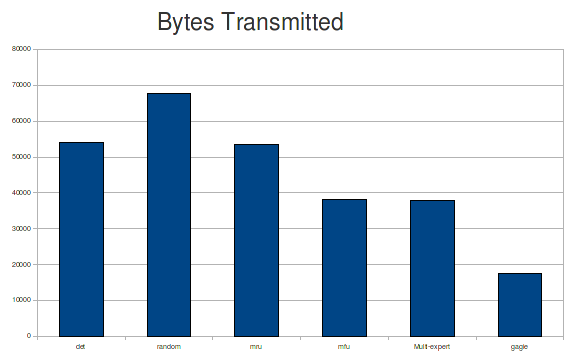
\includegraphics[scale=0.5]{images/firehose_tx.png}
\caption{Bytes Transmitted by the Client}
\label{fig:tx}
\end{figure}

\begin{figure}[!t]
\centering
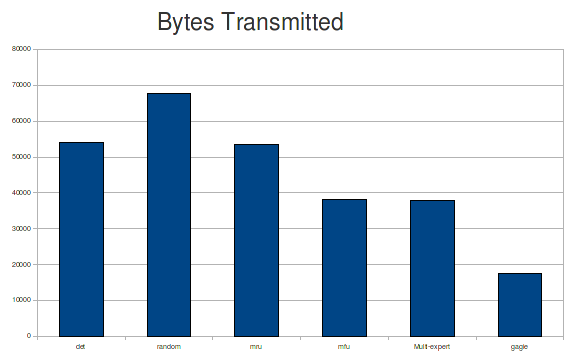
\includegraphics[scale=0.5]{images/firehose_tx.png}
\caption{Bytes Received by the Client}
\label{fig:rx}
\end{figure}

Figs. \ref{fig:tx} and \ref{fig:rx} show the firehose in the best light we were
able to cast on it, and still both images show it to have no hope of achieving
actual energy savings.  It sends more bytes than were in the original file 
even with a weighted multi-expert guess model, while receiving five times
the amount of data in the original file.  With the random guess model, the
firehose protocol sends double the data in the original file, and receives
nearly ten times the amount of data it was attempting to send.

\subsection{ACK Compression}

In a final attempt to lower the amount of data being transmitted by 
the client, we saved all of the ACKs sent by the client out to a file and
then applied numerous compression algorithms (lzo, gzip, bzip2, lzma, 
and our own two-pass range encoder) to them to simulate the online
compression of ACKS.  While some of these compressed file did dip below the 
size of the original file to be sent, none of the were able to beat the 
size of the file when compressed, indicating that, in the interests of 
energy savings, we would have been better off using our processor's power
to encrypt the file initially.

\section{Conclusion}

Here we have presented our findings from our implementation of firehose 
protocol.  Though we initially had hope of achieving a reduction in data
sent by the client through having the server guess the data being sent, due to
the sending of implicit NACKs, such hopes could not be realized.  We attempted
to increase the efficiency of the firehose by implementing 8 different expert 
guessing models on the server, three methods of ACK encoding on the client, 
and even compression of ACKs sent by the client.  None of these attempts could
generate promising results in our experiments.

Fundamentally, as the theoretical works we covered have demonstrated,
entropy of the message determines the number of bits that must be sent
by the client, and the ratio of the speeds of the links is not
a determining factor.

%\bibliographystyle{IEEEtran}
%\bibliography{firehose}
\end{document}
